\section{Data set}

The ASK corpus (\emph{andrespråkskorpus}) was presented in 2006
\autocite{tenfjord06}. The corpus contains Norwegian learner essays from two
different language tests: \emph{Språkprøven i norsk for voksne innvandrere}
and \emph{Test i norsk – høyere nivå}, which test proficiency at the B1 and B2
levels, respectively. Among the metadata included in the corpus
is the learners' L1s, which
are one of German, Dutch, English, Spanish, Russian, Polish,
Bosnian-Croatian-Serbian, Albanian, Vietnamese and Somali. It
provides proficiency labels (in CEFR levels) for all essays from seven of the
L1 backgrounds. The CEFR labels are available since work by
\textcite{carlsen2012proficiency}, and were not included at the corpus'
initial release. Other information included with the documents are which level
of testing they stem from, what topic the essay is about, country of origin, age,
gender and more.

The ASK corpus contains 1700 texts, and 1212 of these have been assigned a
CEFR score. In particular, all texts except those written by people with
Dutch, Bosnian-Croatian-Serbian or Albanian as L1 have a CEFR score.

The corpus contains over 1,127,000 tokens and more than 768,000 words. The
mean word count per essay is therefore higher in ASK than in TOEFL11.


\section{Data split}

At the start of the project, the dataset was split into a training set and a
test set in a 90:10 proportion. Ideally, the train and test sets would have
the same distribution of classes, but the limited amount of data made this
more difficult. As can be seen from figure \ref{lang-vs-cefr}, 15 of the
combinations \(L\times C\) have three or fewer occurences.

\begin{figure}
  \centering
  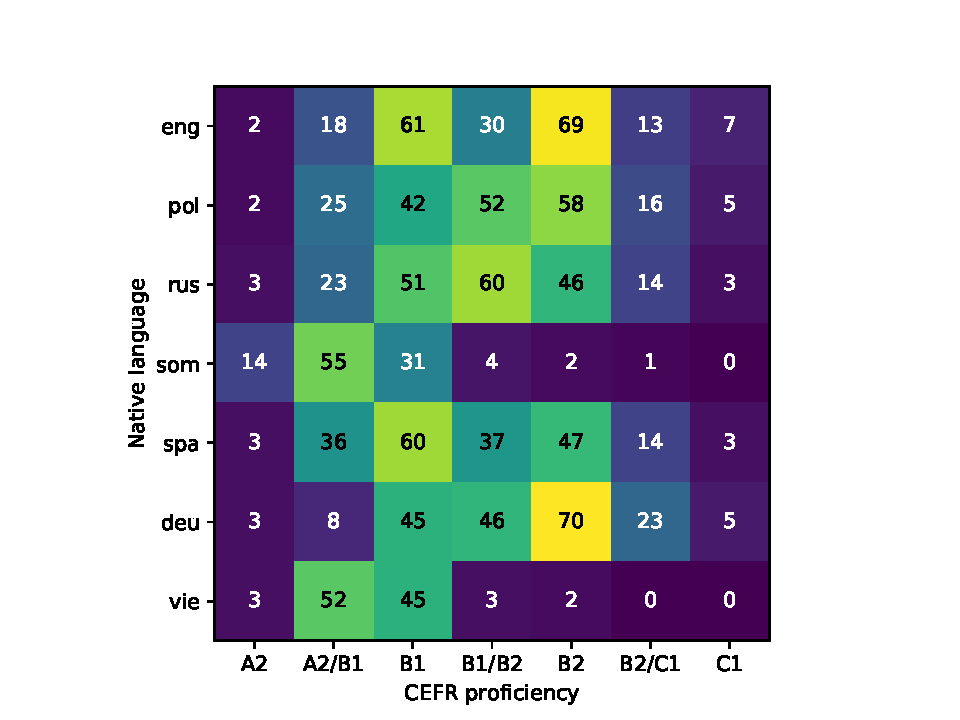
\includegraphics[width=0.8\textwidth]{lang_vs_cefr}
  \caption{The distribution of proficiency scores for each L1}
  \label{lang-vs-cefr}
\end{figure}
 
\begin{figure}
  \centering
  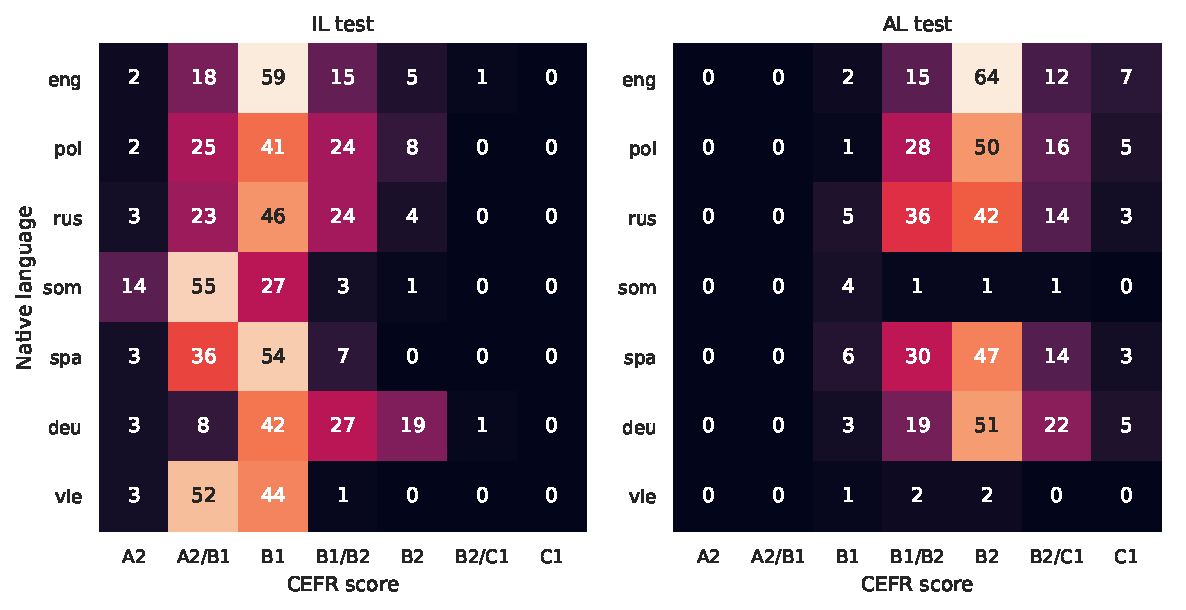
\includegraphics[width=0.8\textwidth]{testlevel_lang_vs_cefr}
  \caption{L1 versus CEFR score for each test level}
  \label{testlevel-lang-vs-cefr}
\end{figure}
 
\subsection{Metadata}

Analysis of the data set was carried out in order to find correlations
between different metadata. Knowing that the documents stem from two
different language tests that measure different levels of proficiency, the
data set was split into two along the \emph{Test level} label, and then broken
down by language and proficiency again. Figure \ref{testlevel-lang-vs-cefr}
shows that the test levels have different distributions of proficiency. Note
also that two language groups are underrepresented at the B2 test level
(``Høyere nivå''), namely Somali and Vietnamese, which have seven and five
essays in the B2 test level, respectively. All other combinations of L1 and
test level contain exactly 100 essays. This partly explains the low average
proficiency of Somali and Vietnamese speakers apparent in figure
\ref{lang-vs-cefr}. The difference compared to the other language groups is
not as salient when looking only at the B1 test level (``Språkprøven'') data.
